\chapter{Problem analysis}\label{cha:problemanalysis}
This chapter details the problem analysis, from the initial problem to a problem statement. Based on the initial problem, a set of questions to research during the problem analysis has been determined:

\begin{description}
    \item[Arduino] What is Arduino, and who uses it? What is the Arduino programming language?
    \item[Concurrency] What is concurrency, and what does it mean to work concurrently? What are the different approaches/models for concurrency, and what are the challenges in relation to Arduino?
\end{description}

\section{Arduino}\label{sec:arduino}
Arduino is an open-source electronics platform that enables users to quickly create small microcontroller projects through easy-to-use hardware and software \cite{WhatArduino}. Multiple variants of Arduino boards exist, with different components and specifications. The UNO, Due, Mega2560, Micro, Leonardo, Zero, Mini, and UNO WiFi are within the classic family of Arduino boards. Because of Arduino being an open-source project, other companies are free to use the specifications to provide third-party implementations of the boards.

\todo{Kig på første sætning}
An Arduino UNO is used as the reference board for this project because \gls{aau} has provided one. All physical tests and examples will run on this board, and the implementation will depend on the Arduino UNO specification henceforth.

The software for the Arduino is the official Arduino IDE, in which developers can write code in the Arduino programming language. The IDE and the programming language is built on Wiring, which builds on Processing \cite{WhatArduino,WiringOrg}.

\subsection{The Arduino programming language}\label{subsec:arduinoprogramminglanguage}
The Arduino programming language closely resembles the C programming language and is, in fact, a set of C/C++ functions \cite{ArduinoSupportC}. It contains most of the constructs of C++, with some additional functions added and a few features, turned off in the compiler, such as exceptions \cite{Nongnuorg}.

\subsubsection{Sketches}
A program written in the Arduino IDE and programming language is called a sketch. A sketch follows a basic structure that consists of implementing the procedures "setup()" and "loop()". Setup is a procedure called once during a run - when the Arduino is turned on or reset; it initializes variables, pin modes, libraries, and some additional links. After setup, the loop begins. The loop procedure is a loop that runs for the duration of the runtime of the program and contains the logic of the project \cite{ArduinoLanguage}.

\subsection{Who uses the Arduino?}\label{subsec:whouses}
A wide range of people, such as students, hobbyists, children, programmers, and professionals, use Arduino for many different purposes \cite{WhatArduino}. Some are focused on the learning aspects of the Arduino - architecture, code, and embedded systems, while others are more interested in designing product concepts. Students and children can use the board to learn the basics of electronics; hobbyists may use it to build personal \gls{diy} projects, while professionals often use it to design product concepts \cite{WhatArduino}.

Designing a programming language for dedicated programmers or professionals may require a profound understanding of many underlying details of the Arduino platform itself. Providing a good language for these groups can potentially detract from the project's purpose - which is to design a programming language - because it may take more time than is available to obtain this knowledge. Thus, this is not the target group. The project also will not deal with a programming language designed for children, as this would require an understanding of pedagogical tools, which is outside the scope of a computer science education.

The hobbyist is, however, an excellent group for which to design our implementation for. Because hobbyists spend their leisure time on Arduino projects, the primary concerns are their limited available time and the potential for frustration during a project. Moreover, hobbyists might have limited programming proficiency or be complete beginners. The standard Arduino language already alleviates many problems, but not in regards to concurrency. The user group for the remainder of this report is hobbyists who want to do as much as they can with their limited time and limited coding proficiency - specifically related to concurrency.
\section{Concurrency}\label{sec:concurrency}
The term concurrency is a general term for ways a computer system performs multiple tasks simultaneously. It covers the \textit{simulation} of multiple tasks running at the same time through process switching, as well as work done in parallel. To disambiguate, based on the definition:

\blockcquote{Bryant2016}{We use the term concurrency to refer to the general concept of a system with multiple, simultaneous activities, and the term parallelism to refer to the use of concurrency to make a system run faster.}

We infer that parallelism is a type of concurrency to speed up the system, while concurrency, in general, may have purposes not related to speed, for example, synchronization of tasks.

Concurrency is a complex, large, and hardware-dependent subject~\cite{Sebesta2016}. The limitations of the Arduino hardware concerning concurrency, specifically the \gls{cpu}, are explored before concurrency in general because the project is, first and foremost, about programming language design - not concurrency.

\subsection{Arduino hardware}\label{subsec:arduinohardware}
The Arduino Uno board uses the ATmega328P microcontroller~\cite{ArduinoUno}. The architecture of this microcontroller is a scalar single-core processor without hyperthreading(intel) or \gls{smt} (AMD) equivalents~\cite{ATmega328P}.

Since there only exists a single core, which does not contain any duplicate copies of CPU hardware (for multithreading), the only hardware parallelism on the Arduino Uno is instruction-level parallelism, and only to the level of up to 1 instruction per clock cycle (scalar). This parallelism is also handled directly by the \gls{cpu} and does not impact the instruction set available to developers.


\begin{figure}[htb!]
    \centering
    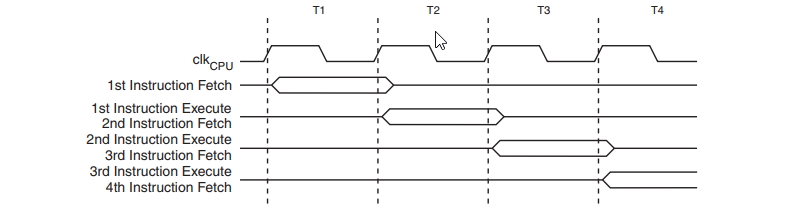
\includegraphics[width=\textwidth]{figures/Arduino_Pipeline.png}
    \caption{The parallel intruction fetches and intruction executions \cite{ATmega328P}}
    \label{fig:arduinopipeline}
\end{figure}


Therefore, the Arduino is a uniprocessor~\cite{Bryant2016} whose architecture does not support parallel processing - and for the remainder of the report, the term concurrency refers to concurrency \textbf{without parallelism}.

Even unicore processors can support several models for concurrency at the application software level, which makes sense since most computers often have more processes running than \glspl{cpu}. Achieving this concurrency is done through interleaving instructions of different processes, which lets the \gls{cpu} appear to run multiple programs.

This interleaving is commonly handled by an \gls{os}, which manages the hardware resources~\cite{Bryant2016}. However, by default, the Arduino does not have an \gls{os}. It is still possible to achieve concurrency on an Arduino, but not without a scheduler or scheduling.

\subsection{Concurrency on an Arduino}\label{subsec:concurrencyinarduino}
The scheduler is the part of the \gls{os} that handles the planning and switching of different tasks on the CPU within the system. However, an \gls{os} is not the only way to obtain scheduling behavior. Several online tutorials~\cite{BadExample1, BadExample2} demonstrate different techniques to achieve concurrency on an Arduino, such as using the Arduino functions millis() and interrupt().

The millis() technique executes different pieces of code depending on some programmer-defined timeslices and comparisons between the current time and an earlier time. The interrupt() method uses the \gls{cpu} interrupt command to interrupt the \gls{cpu} and restart it from another place in the code.

Both methods require the programmer to think deeply about how they wish for the program to execute, which can get complicated and frustrating fast. The interrupt() case is a very low-level command that might not work entirely as a novice or hobbyist expects. In the case of the millis() method, it requires many global variables to execute the program correctly, which can be difficult. In both cases, the code may be hard to maintain or understand.

These examples highlight a general difficulty with the Arduino model, and several solutions to the described problems exist, some of which are explored in the next section.

\section{Existing solutions}\label{sec:existingsolutions}
In this section, some ways of achieving concurrency on an Arduino is explored. Emphasis is put on the immediate advantages and disadvantages related to each model, when considering the impact on the hobbyist users, by which is meant the new challenges, if any, introduced by the model in question.

A small sample project is implemented in each model for the sake of comparison: The builtin \gls{led} of the Arduino is set to blink - turn on and off - every half second. Concurrently, the state of a button is read and printed continously. The example will be implemented in the Arc programming language as well. The schematic for the project is seen in Figure ~\ref{fig:exampleprojectschematic}.


\begin{figure}[htb!]
  \centering
  \missingfigure[figwidth=0.8\textwidth]{Insert image of Arduino schematic?}
  %\includegraphics[width=0.8\textwidth]{example-image-a}
  \caption{Example project schematic}
  \label{fig:exampleprojectschematic}
\end{figure}


The first discussion is about the prospect of using programming libraries to achieve concurrency on an Arduino. The second discussion is about the possibility of installing an \gls{os} on the Arduino, and building on the \gls{os}-exposed concurrency abstractions.

\subsection{Concurrency through Arduino libraries}\label{subsec:arduinolibraries}
In this section, the \textit{Protothreads} and \textit{Eventually} libraries are explored and compared. Of particular concern is the quality of the documentation, the model of concurrency, and the overhead of usage on the Arduino.

\subsubsection{Protothreads}
Protothreads is a library for the C language, which has been implemented as a library for Arduino \cite{Artin2020}. It is based on Adam Dunkels protothreads ~\cite{AdamDunkelProtothreads}.


\blockcquote{Artin2020, AdamDunkelProtothreads}{Protothreads provides a blocking context on top of an event-driven system, without the overhead of per-thread stacks. The purpose of protothreads is to implement sequential flow of control without complex state machines or full multi-threading.}


\begin{listing}[htb!]
  \centering
  \begin{minted}[label=Protothreads example]{arduino}
    #include "protothreads.h"
    const int buttonPin = 12; const int ledPin = 8;
    int buttonState = 0;  // variable for reading the pushbutton status
    pt ptBlink, ptButton;

    int blinkThread(struct pt *pt) {
      PT_BEGIN(pt);
      for (;;) {
        digitalWrite(ledPin, HIGH); // turn the LED on (HIGH is the voltage level)
        PT_SLEEP(pt, 500);
        digitalWrite(ledPin, LOW); // turn the LED off by making the voltage LOW
        PT_SLEEP(pt, 500);
      }
      PT_END(pt);
    }

    int buttonThread(struct pt *pt) {
      PT_BEGIN(pt);
      for (;;) {
        buttonState = digitalRead(buttonPin);
        Serial.println(buttonState);
        PT_YIELD(pt);
      }
      PT_END(pt);
    }

    void setup() {
      PT_INIT(&ptBlink);
      PT_INIT(&ptButton);
      Serial.begin(9600);
      pinMode(ledPin, OUTPUT);
      pinMode(buttonPin, INPUT);
    }

    void loop() {
      PT_SCHEDULE(blinkThread(&ptBlink));
      PT_SCHEDULE(buttonThread(&ptButton));
    }
  \end{minted}
  \caption{A small example on how a Protothreads can be implemented}
  \label{lst:protothreadsexample}
\end{listing}


The pitch for Protothreads is promising, and directly addresses the concern about overhead. However it does not describe the model of concurrency in great detail. Fortunately the documentation is excellent on both the Arduino implementation ~\cite{Artin2020} as well as the general Protothreads specification ~\cite{AdamDunkelProtothreads}.

Protothreads uses a cooperative form of concurrency, which means it is us tp the user to synchronize the program. This means that a program written with protothreads is event-driven and blocking - it must finish, or pause, explicitly, before moving on to the next task.

Protothreads is also implemented on a single stack with stack rewinding, unlike traditional multithreadings which has a stack per thread. This is the reason for the low overhead of Protothreads. On the Arduino, this is achieved through utilization of \textbf{local continuations} - threads are simply a struct with an unsigned short - together with macros that expand to a switch statement with a number of returns. The short contained in the thread is the set and compared against the switch defined by the macros to set the state and continuation.

Because threads are a struct with a short, they have a size of only two bytes. This means that there is no hidden memory cost during the execution of the program. However, the implementation details of the Protothread library does have a few effects on how to write programs when using it. 

First, a protothread only saves the short across blocking calls. This means that local variables inside a thread are not preserved - a rule of thumb from the designer is that local variables simply should not be used inside a protothread. Instead, it is prudent to use global variables, if data should be preserved.

% BEGIN HERE FRIDAY
Secondly, the scheduling of protothreads uses a switch statement in a way that prevents 




Lastly, it is important that the code inside a Protothread needs to be "fast", meaning that the programmer should not use any of the arduino cpu blocking functions, such as the delay() function, because this would block the other functions to run. ~\cite{AdamDunkelProtothreads}

The implementation of our sample project with protothreads can be seen in Listing ~\ref{lst:protothreadsexample}.






%---Links to Eventually c++ Libary---
%1. https://github.com/johnnyb/Eventually
%2. https://www.arduino.cc/reference/en/libraries/eventually/
% What is Eventually C++ Library?
% Advantages and disadvantages of Eventually Library (C++ issues)

\subsubsection{Eventually}
% From what I have found there is basic two valid sources which shortly explain what the Eventually C++ Library is and then there is some smaller code examples that show how to use it. So i don't know how relevant it is to have in the report since is just an other way of making event-bases programming like protothreads?
Eventually is an Arduino Event-based Programming Library. Where the goal is to make a more event-oriented environment for the Arduino programming language.

To give a better understanding of how the Eventually C++ library is working, in this section there has been taken an example from a GitHub page ~\cite{bartlettEventually2022Bartlett} where there can be seen, a code example on how to use the Eventually library. Since it is a C++ library it would work on any Arduino board, which includes the one the group has acquired.


\begin{listing}
  \begin{minted}[label=Eventually example]{arduino}
    #include <Eventually.h>
    #define LIGHT_PIN 8
    #define BUTTON_PIN 12
    bool pinState = true;
    EvtManager mgr;

    bool blinker() {
      mgr.resetContext();
      mgr.addListener(new EvtTimeListener(1000, true, (EvtAction)blink_pin)); 
      mgr.addListener(new EvtPinListener(BUTTON_PIN, (EvtAction)digital_read));
    }

    void blink_pin() {
      if (pinState == true) {
        digitalWrite(LIGHT_PIN, HIGH);
      } else {
        digitalWrite(LIGHT_PIN, LOW);
      }
      pinState = !pinState;
    }

    void digital_read() {
        int sensorVal = digitalRead(BUTTON_PIN);
        Serial.println(sensorVal);
        delay(1);
    }

    void setup() {
      Serial.begin(9600);
      pinMode(LIGHT_PIN, OUTPUT);
      pinMode(BUTTON_PIN, INPUT);
      blinker();
    }

    USE_EVENTUALLY_LOOP(mgr)
  \end{minted}
  \caption{A small program on how Eventually can be implemented}
  \label{lst:eventuallyexample}
\end{listing}


\subsection{Achieving Concurrency with an Operating System}



%---Links to Free rtos---
%1. https://github.com/feilipu/Arduino_FreeRTOS_Library
%   Forklar hvad link går ud på
\subsubsection{FreeRTOS}
Free Real-Time Operating System (abbreviated to FreeRTOS) is an operating system specifically designed for microcontrollers and microcomputers, such as the Arduino. It has been developed in partnership with the leading chip companies in the world, over more than 18 years, and with a special emphasis on reliability, accessibility and ease of use ~\cite{AboutRTOS}. This leads itself well to our project, while we are targeting hobbyists. FreeRTOS utilises preemptive scheduling ~\cite{SchedulingRTOS}, which means that it implements a scheduler to be responsible for deciding which tasks to do in which order.



\begin{listing}[htb!]
  \centering
  \begin{minted}[label=FreeRTOS example]{arduino}
#include <Arduino_FreeRTOS.h>

void TaskBlink(void *pvParameters){ // This is a task.
  (void) pvParameters;
  pinMode(LED_BUILTIN, OUTPUT);
  for (;;) { // A Task shall never return or exit.
    digitalWrite(LED_BUILTIN, HIGH);
    vTaskDelay( 1000 / portTICK_PERIOD_MS );
    digitalWrite(LED_BUILTIN, LOW);
    vTaskDelay( 1000 / portTICK_PERIOD_MS );
  }
}

void TaskAnalogRead(void *pvParameters){ // This is a task.
  (void) pvParameters;
  for (;;) {
    int sensorValue = digitalRead(12);
    Serial.println(sensorValue);
    vTaskDelay(1);
  }
}

void setup() {
  Serial.begin(9600);
  while (!Serial) {;}
  xTaskCreate(TaskBlink, "Blink", 128, NULL, 2, NULL);
  xTaskCreate(TaskAnalogRead, "AnalogRead", 128, NULL, 1, NULL);
}

void loop(){}
\end{minted}
  \caption{A small example of a possible implementation of Free RTOS.}
  \label{lst:freeftosexample}
\end{listing}

%and Preemptive concurrency forms \cite{UsingFreeRTOSMultitasking}, the preemptive concurrency form is priority-based, like the cooperative concurrency form the preemptive concurrency form has to prioritise the tasks in the program, but a task has to be completed in the time period which the scheduler has given task, it then switches to another task and if the first task was not completed it switches back \cite{Windows}.
%the library has a scheduler to set up when the tasks have to be executed, the programmer can also set up when the Arduino has to do a specific task, if no specific timed workflow, the scheduler assigns the priority of the tasks \cite{UsingFreeRTOSMultitasking}. 

%---Links to Simba library---
% 1. https://simba-os.readthedocs.io/en/latest/
%   Forklar hvad link går ud på
% 2. https://all3dp.com/2/best-arduino-operating-system/
%   Forklar hvad link går ud på
%\subsubsection{Simba}



%---Links to TaskManagerIO library---
% 1. https://github.com/davetcc/TaskManagerIO
%   Forklar hvad link går ud på
% 2. https://all3dp.com/2/best-arduino-operating-system/
%   Forklar hvad link går ud på
%\subsubsection{TaskManagerIO }




It is also possible to install an \gls{os} on the Arduino, and obtain a scheduler (and other things) that way.

\subsection*{Deprecated at the moment}
\subsection{Models of concurrency}\label{subsec:modelsofcon}
% might be relevant to explain the concurrency models of an OS, to compare the choices.
This interleaving is commonly handled through an \gls{os}, which manages the hardware resources ~\cite{Bryant2016}. A few different approaches for interleaving processes are supported by most \glspl{os}:

\subsubsection{Processes}
In this model the kernel, the portion of the \gls{os} code that resides in memory while the system is running, schedules and maintains each logical control flow, called a process. Each process has its own virtual address space, and therefore requires a mechanism for interprocess communication ~\cite{Bryant2016}.

\subsubsection{I/O multiplexing}
When an application explicitly schedules its own logical control flow, in the context of a single kernel process, you have I/O multiplexing. In the application, each logical control flow is modelled as a state machine, with the transitions defined and managed by the application code. Since this model is a single process, control flows share virtual address space ~\cite{Bryant2016}.

\subsubsection{Threads}


\subsection{Summary}



\section{Problem statement}\label{sec:problemstatement}
\textit{Concurrency} is a complex subject that has to be studied deeply by programmers~\cite{Sebesta2016}. It cannot be expected for a hobbyist to study concurrency in its entirety for hobby projects - unless they are programmers or computer scientists - the scope is too large for most hobbyist projects.

Many languages include constructs to abstract some concurrency details away, making it easier to write concurrent programs. The Arduino programming language does not, which complicates writing concurrent programs in the Arduino language.

For these reasons, hobbyists often face many difficulties when writing concurrent programs for the Arduino, which may be solved easily in other programming languages. Therefore the problem statement for this project is as follows:

\blockquote{Creating a programming language for the Arduino with concurrency constructs leveraging the Protothreads library to express a concurrent flow of control concisely.}



%To create a programming language for the Arduino, that leverages the Protothreads library to concisely express a concurrent and intuitive flow of control.

%\blockquote{To create a programming language with superficial and easy to understand and use constructs, that can be used to concisely express }

%To create a programming language for the Arduino, with easy to understand and use constructs, that can be used to concisely express concurrent 

%\blockquote{To create an extension on the Arduino programming language to support concurrency in real-time systems. The language should aid hobbyists in writing idiomatic Arduino programs.}

%\blockquote{To create a programming language for Arduino, which leverages some concurrency mechanism, to make it simpler or easier for hobbyists to write idiomatic Arduino programs with concurrency.}

%\blockquote{To create a programming language for Arduino, which leverages some concurrency mechanism, to make it simpler or easier for hobbyists to write idiomatic Arduino programs with concurrency.}